%************************************************
\chapter{Introduction}\label{ch:introduction}
%************************************************

Any rhythmic motor behavior necessary to life must be stable under environmental perturbation, yet sensitive to internal cues from the organism. Respiration, for instance, must continue interminably, but must also be able to account for the holding of one's breath against noxious stimuli or increase in amplitude or frequency during exercise. 

Many rhythmic behaviors begin as activity in central pattern generators (\acsp{CPG}), neuronal circuits which intrinsically produce rhythmic motor patterns in the absence of sensory or descending inputs\autocite{MarderCentralpatterngenerators2001}. A central pattern generator must be robust to environmental perturbation to avoid losing rhythmicity. Simultaneously, it must be responsive to intended modulation from within the organism. In respiration, for instance, serotonin neuromodulation maintains \acs{CPG} activity in respiration; disruption of neuromodulation can result in hypoxia or death\autocite{DoiNeuromodulationOrchestrationRespiratory2008,PenaEndogenousActivationSerotonin2A2002}. The interplay between stability and sensitivity permit the same circuit to produce multiple outputs as a response to endogenous modulation\autocite{Nusbaumrolescotransmissionneural2001}.

Neuronal circuits which are not tightly tuned are degenerate; there are many solutions, viable sets of parameters, which produce similar network output\autocite{TononiMeasuresdegeneracyredundancy1999,EdelmanDegeneracycomplexitybiological2001,WhitacreDegeneracydesignprinciple2010,DrionIonchanneldegeneracy2015}. For stable and responsive biological activity, degenerate networks must still be robust to environmental perturbation and responsive to intentional modulation. In this thesis, I describe red pigment-concentrating hormone (\acs{RPCH}) acting as a neuromodulator on a computational model of a rhythmic motor circuit.

\section{The Stomatogastric Ganglion}
The stomatogastric nervous system (\acs{STNS}) provides an excellent model system for analyzing how circuit dynamics arise from neuronal properties and network connectivity\autocite{MarderPrinciplesrhythmicmotor1996}. Initial work began in the 1970s using the \acs{STNS} to understand central pattern generation\autocite{MaynardSimplernetworks1972,HartlinePatterngenerationlobster1979,RaperNonimpulsemediatedsynaptictransmission1979}. Several properties make this system ideal for electrophysiological and computational analysis.

The \acs{STNS} consists of a group of four linked ganglia: the paired commissural ganglia (\acs{CoG}), the oesophageal ganglion (\acs{OG}), and the stomatogastric ganglion (\acs{STG})\autocite{SelverstonCrustaceanStomatogastricSystem1987,Harris-WarrickDynamicBiologicalNetworks1992}. Each of the \acsp{CoG} contains approximately 400 neurons and the \acs{OG} contains approximately 18 neurons. The stomatogastric ganglion (\acs{STG}) is comprised of approximately 30 neurons – the exact number varies between species and between animals. In the healthy animal and \textit{in-vitro} preparation, the \acs{STG} produces a triphasic motor rhythm with a frequency of about 1 Hz\autocite{MarderCentralpatterngenerators2001,MarderRobustcircuitrhythms2015}. When pharmacologically isolated, most \acs{STG} neurons fire tonically but can be induced to conditionally burst  under the influence of neuromodulators or graded inhibitory input\autocite{MarderNeuromodulationNeuronalCircuits2012}.

\begin{figure}[h]
	\centering
	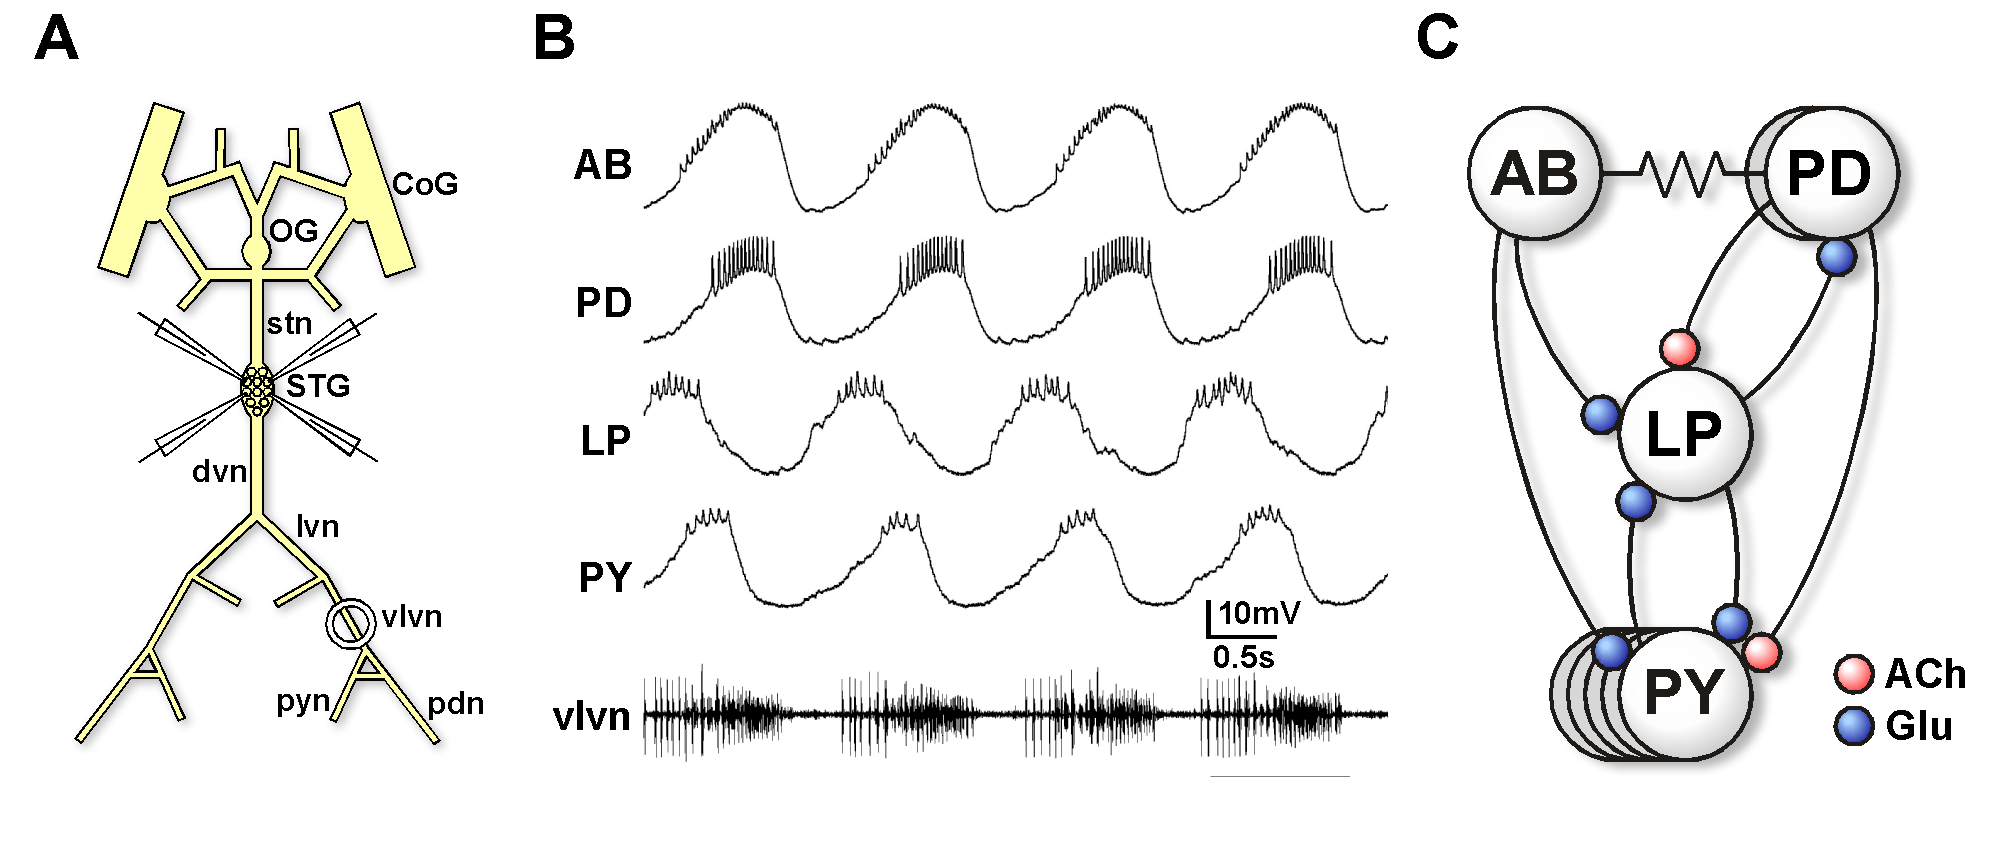
\includegraphics[width=1.0\linewidth]{gfx/PyloricRhythm}
	\caption[The stomatogastric ganglion]{The stomatogastric ganglion. (\textsc{A}) Diagram of the \acs{STNS} showing the ganglia (capitals) and the major nerves (lowercase). (\textsc{B}) Intracellular recordings from four cells in the pyloric circuit of the \acs{STG}. The fifth trace shows extracellular \textit{vlvn} nerve recording, which contains potentials from the above cells. (\textsc{C}) Circuit diagram showing synaptic connectivity in the pyloric circuit. Resistor symbols indicate electrical synapses. \textsc{ACh} are acetylcholinergic and \textsc{Glu} are glutamateric synapses, where balls indicate post-synaptic targets\autocite{NusbaumMichaelP.Functionalconsequencesneuropeptide2017}.}
	\label{fig:pyloricrhythm}
\end{figure}


\acs{STG} neurons have large somata (typically 50-100 microns across) and complex dendritic morphology\autocite{OtopalikSloppymorphologicaltuning2017,CuntzOnerulegrow2010}. While these cells possess long axons which contribute to descending nerves, much of the arborization consists of neurites which tangle extensively in the neuropil. This wiring follows a space-filling mechanism. Despite this tangled morphology, \acs{STG} neurons are electronically compact. Gradations in reversal (Nernst) potential as a function of path distance from the soma maintain signal amplitude near and far from zones of integration\autocite{OtopalikSloppymorphologicaltuning2017}. Therefore, the circuit relies on intrinsic and synaptic properties instead of morphological tuning to produce network activity.

Robustness to mechanical insult permits dissection and electrophysiological recording \textit{in-vitro}. The fictive motor patterns produced by the \acs{STG} survive for at least 24 hours without incubation and are representative of both the activity of the circuit \textit{in-vivo} and the motor output\autocite{HamoodConsequencesacutelongterm2015}. Additionally, since most synaptic connections in the \acs{STG} occur between motor neurons, the circuit can be isolated from descending interneurons\autocite{HamoodQuantitativeReevaluationEffects2015,GoldmanGlobalStructureRobustness2001,HaddadCircuitrobustnesstemperature2017}.  Decentralization by severing the \textit{stn}, the descending nerve which connects the \acsp{CoG} and \acs{OG} to the \acs{STG}, removes descending neuromodulation.

\begin{figure}[h]
	\centering
	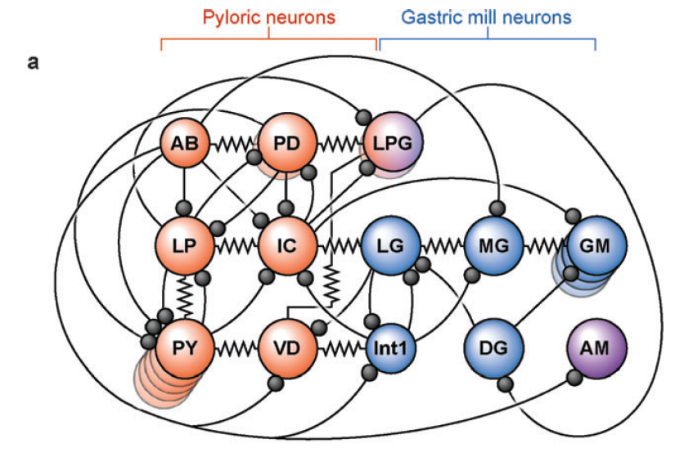
\includegraphics[width=1\linewidth]{gfx/NusbaumMarder2017.png}
	\caption[Circuit diagram of the STG]{Circuit diagram of the stomatogastric ganglion (\acs{STG}). Circles are neurons, resistor symbols are electrical synapses, balls indicate post-synaptic inhibitory targets.\autocite{NusbaumMichaelP.Functionalconsequencesneuropeptide2017}.}
	\label{fig:circuitdiagram}
\end{figure}

\FloatBarrier


\section{The Pyloric Rhythm}
The pyloric rhythm is a triphasic motor pattern almost always continuously expressed in the healthy crustacean\autocite{ClemensLongtermexpressiontwo1998,RezerExpressioncrustaceanpyloric1983}. The frequency of the rhythmic behavior may vary over $[0.5, 2.5]$ Hz, but the burst order, phase relationships, and duty cycle are maintained in healthy animals\autocite{MarderUnderstandingCircuitDynamics2007}. The canonical pyloric rhythm consists of bursts of action potentials in the pyloric dilator (\acs{PD}) neurons, followed by bursts in the lateral pyloric (\acs{LP}) neuron, and finally by bursts in the pyloric (\acs{PY}) neurons. The inferior cardiac (\acs{IC}) neuron fires often with the (\acs{LP}) neuron and the ventricular dilator (\acs{VD}) neuron fires frequently with the PY neurons\autocite{Harris-WarrickDynamicBiologicalNetworks1992}. The anterior burster (\acs{AB}) interneuron projects through the stomatogastric nerve to the \acsp{CoG} and is electrically coupled to the twin \acs{PD} neurons. 

In normal pyloric activity, the \acs{AB} neuron intrinsically oscillates. The \acs{PD} neurons, electrically coupled to \acs{AB}, burst in phase. The \acs{AB} and \acs{PD} cells inhibit \acs{LP} and \acs{PY}, which both burst during \acs{PD} interphase. \acs{LP} rebounds from inhibition faster than \acs{PY} and bursts first. \acs{LP} and \acs{PY} are in a phase-antiphase ’half-center’ oscillator regime of mutual inhibition (\autoref{fig:pyloricrhythm}). \acs{PY} neurons rebound and inhibit \acs{LP} to terminate bursting in the coupled cell\autocite{MarderUnderstandingCircuitDynamics2007,HooperModulationlobsterpyloric1987,Harris-WarrickDynamicBiologicalNetworks1992}. In this regime, \acs{AB} is considered the intrinsic pacemaker and \acs{AB}-\acs{PD} the pacemaker kernel. Selective photo-inactivation of cell types and glutamate-blocker experiments show that \acs{AB} reliably maintains oscillations while decoupled\autocite{SelverstonCrustaceanStomatogastricSystem1987}. The phaselocking of \acs{LP} and \acs{PY} during \acs{PD} interphase is dependent on the intrinsic and synaptic characteristics of the network. 

The pyloric rhythm is robust to perturbation. The circuit is most stable under physiological conditions (11 deg. C with descending neuromodulatory input), however the STG can maintain the phase differences characteristic of pyloric rhythmicity at temperatures up to 31 deg. C and under long-term decentralization\autocite{HaddadCircuitrobustnesstemperature2017,TangRobustnessrhythmiccircuit2012,HamoodConsequencesacutelongterm2015,GoldmanGlobalStructureRobustness2001}.

While the pyloric rhythm is robust to environmental perturbation, it is also susceptible to neuromodulation, allowing for flexibility in network output while maintaining stability. Neuromodulators are released into the neuropil as a consequence of sensation in the animal or descending modulatory projections from the \acsp{CoG} and \acs{OG}\autocite{MarderNeuromodulationNeuronalCircuits2012,JohnsonAminemodulationglutamate1997,Nusbaumsmallsystemsapproachmotor2002,MarderCentralpatterngenerators2001,Nusbaumrolescotransmissionneural2001}.

 
\begin{figure}[h]
	\centering
	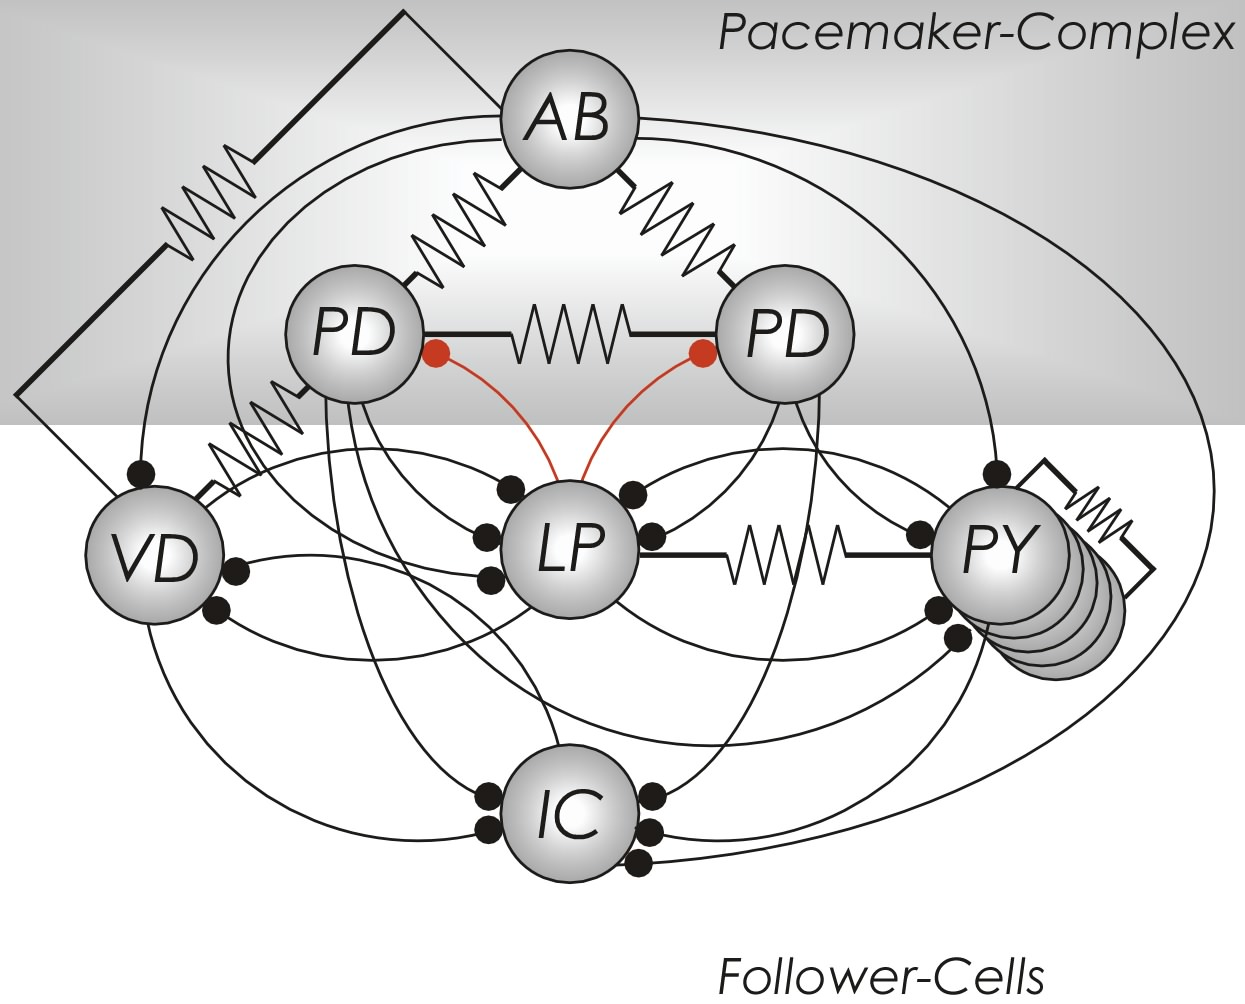
\includegraphics[width=1\linewidth]{gfx/PyloricCircuit}
	\caption[Circuit diagram of the pyloric circuit]{Circuit diagram of the pyloric circuit. Resistor symbols represent electrical synapses, dots represent inhbitory synapses. \acs{AB} and \acs{PD} form the pacemaker kernel.}
	\label{fig:pyloriccircuit}
\end{figure}

The \acs{STG} is multiply-modulated. The pericardial organ and other neurosecretory organs secrete neuromodulators into the neuropil which colocalize in specific neurons. In addition, many hormones circulating in the hemolymph can also act as neuromodulators in the \acs{STG}\autocite{MarderNeuromodulationNeuronalCircuits2012,NusbaumMichaelP.Functionalconsequencesneuropeptide2017,BlitzDifferentProctolinNeurons1999}.

In general, neuromodulators enhance the flexibility of neuronal networks. In one such method, neuromodulators activate a new current \acs{IMI}, a  fast, non-inactivating, voltage-gated inward current which predominately activates between -40 mV and -20 mV\autocite{GolowaschIoniccurrentslateral1992,GolowaschProctolinactivatesinward1992}.

All cells in the pyloric circuit are capable of activating \acs{IMI} through modulatory action, though they vary in its response. Differential receptor expression leads to variability and flexibility in cellular and network response to modulatory chemicals\autocite{SchulzVariablechannelexpression2006,OLearyCorrelationsionchannel2013}.

Application of red-pigment concentrating hormone (\acs{RPCH}) to the \acs{STG} increases the frequency and amplitude of slow-wave oscillations in the pyloric circuit, while phase relationships are maintained\autocite{NusbaumNeuronalRoleCrustacean1988} (\autoref{fig:rosenbaum2}, P. Rosenbaum, unpublished). Thus, the nerves which innervate the pylorus transmit the same patterned activity at the desired frequency, maintaining muscle tonus. 

\begin{figure}[h]
	\centering
	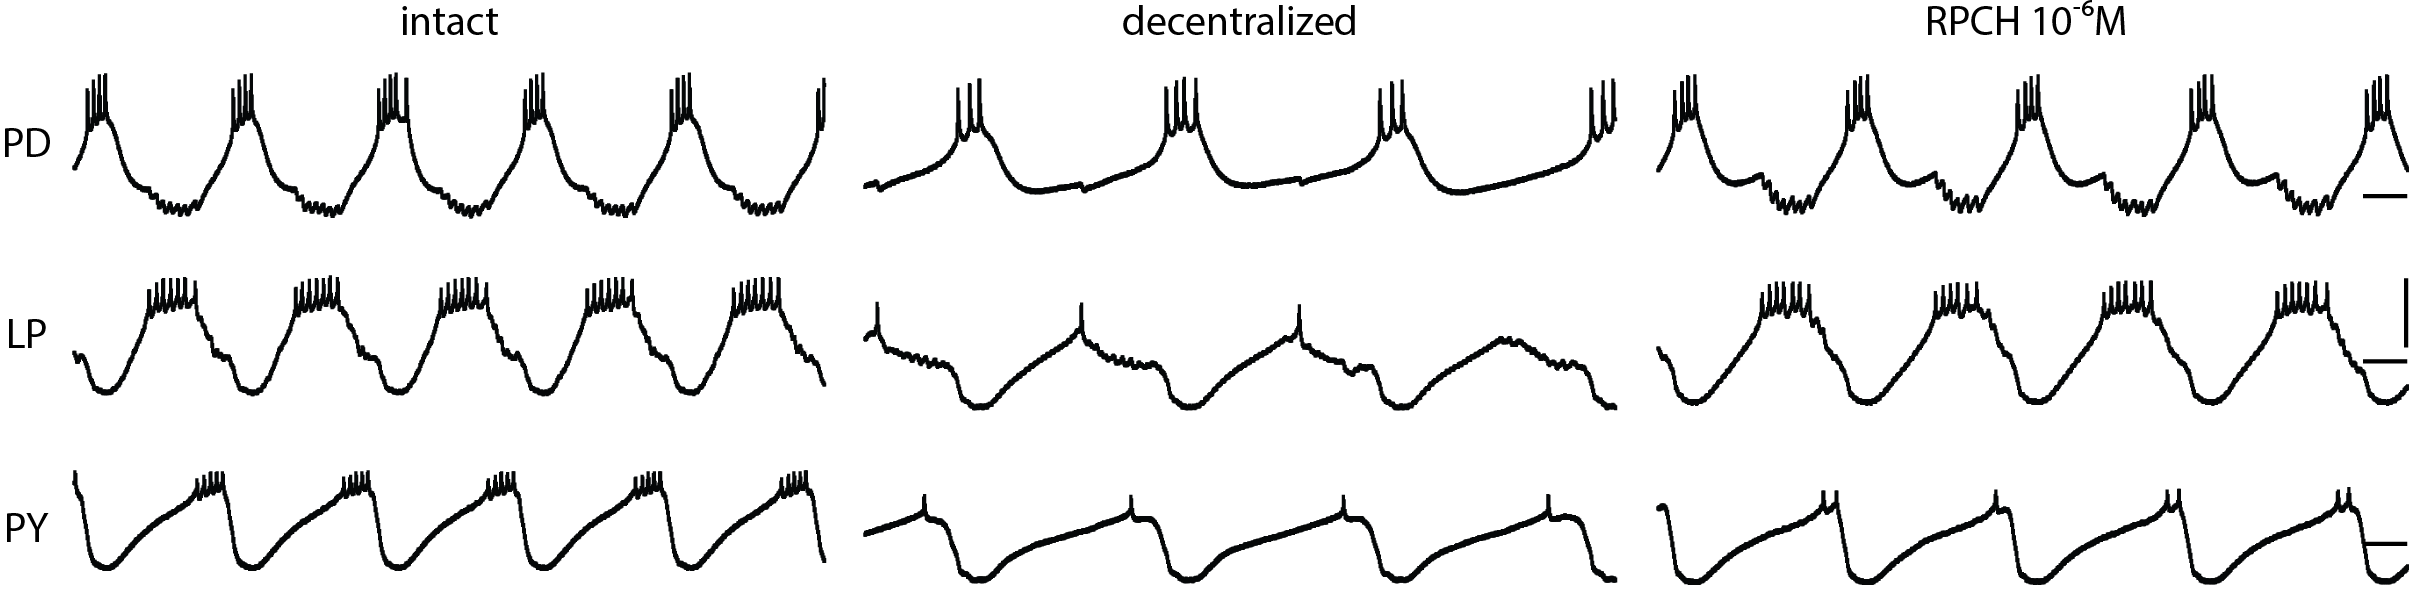
\includegraphics[width=1\linewidth]{gfx/Rosenbaum2}
	\caption[Pyloric Rhythms in \acs{RPCH}]{Pyloric rhythms in \acs{RPCH}. Traces on the left show a regular pyloric rhythm in the intact \acs{STNS}. Intracellular recordings of \acs{PD}, \acs{LP}, and \acs{PY} and an extracellular recording of the \textit{lvn} (lateral ventricular nerve) show the coordinated, triphasic rhythm. The intact rhythm has a frequency of about 1 Hz. Following decentralization (middle trace) the rhythm frequency and spikes per burst in all neurons decreased. After application of 1 $\mu \mathrm{M}$ \acs{RPCH}, the rhythm sped up and spikes per burst increased. Horizontal scale bars denote the membrane potential at -50 mV, vertical scale bars mark 20 mV (P. Rosenbaum, unpublished).}
	\label{fig:rosenbaum2}
\end{figure}

Three models of \acs{IMI} were examined. The first, published in Sharp \textit{et al.}, mimics proctolin in \acs{AB} neurons of \textit{C. borealis} using dynamic clamp\autocite{SharpDynamicclampcomputergenerated1993}. The characteristic increase in burst frequency and slow-wave amplitude under \acs{IMI} is shown in \autoref{fig:sharp2}.

\begin{figure}[h]
	\centering
	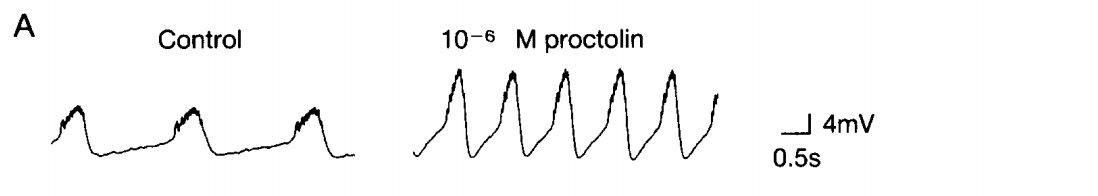
\includegraphics[width=1\linewidth]{gfx/Sharp2}
	\caption[Proctolin on AB neurons]{Proctolin increases amplitude and frequency of \acs{AB} oscillations. Intracellular recording from a lobster \acs{AB} neuron in control saline and 1 $\mu \mathrm{M}$ proctolin.\autocite{SharpDynamicclampcomputergenerated1993}.}
	\label{fig:sharp2}
\end{figure}


Swensen \& Marder fit current-voltage and dosage-response curves to proctolin in \acs{PD} and \acs{PY} neurons\autocite{SwensenMultiplepeptidesconverge2000,SwensenModulatorsconvergentcellular2001}. The \acs{STG} was decentralized from descending neuromodulatory inputs with sucrose block and artificial proctolin current was added via dynamic clamp, based on IV curves.

Soto-Trevi\~no \textit{et al.} developed a model of the pacemaker kernel based on recordings in spiny lobsters\autocite{Soto-TrevinoComputationalmodelelectrically2005}. Neuromodulatory inputs into the AB neuron were modeled by \acs{IMI}. The current was fit to the model, rather than to biological data. The parameters of the current satisfied the constraints that the model would mimic decentralized behavior without the current, and control behavior with the current.

\FloatBarrier

\section{Neurodynamics}
Analysis of high-dimensional conductance-based models form the backbone of this thesis. Each neuron is considered to consist of compartments, each with membrane properties and a collection of ionic and synaptic currents\autocite{AbbottAnalysisNeuronModels1993,Liumodelneuronactivitydependent1998}. The membrane potential $V_m$ of a compartment evolves according to the Hodgkin-Huxley formalism, which envisions excitable membranes as capacitors with variable resistors in parallel\autocite{Hodgkincomponentsmembraneconductance1952}. The membrane potential evolves over time as a function of the sum of the transmembrane currents. This is described by the conservation of current equation for a capacitative membrane.

\begin{equation} \label{eq:voltage}
	C_m \frac{\mathrm{d}V_m}{\mathrm{d}t} = - \sum_i I_i
\end{equation}

where $C_m$ is the membrane capacitance and $I_i$ each current. Each current is described as non-Ohmic with conductance $g$.

\begin{align}
	I_i(V_m) =&\ g_i(V_m)(V_m-E_i) \\
	g_i(V_m) =&\ \bar{g}_i m_i^{p_i} h_i^{q_i}
\end{align}

where

\begin{tabular}{ll}
	$\bar{g}$    & maximal conductance \\
	$m$     	 & activation gating variable \\
	$h$          & inactivation gating variable \\
	$p,q$        & integer exponents \\
	$E$          & reversal (Nernst) potential \\
\end{tabular}

The gating variables $m$ and $h$ are bounded in $[0, 1]$ so that the effective conductance $g_i(V_m)$ from the $i^{th}$ conductance lies between zero and the maximal conductance. When $m=0$, no channels of that conductance are open; when $h = 0$, all channels of that conductance are inactivated.

The gating variables evolve with time

\begin{equation}
	\tau_x(V_m) \frac{\mathrm{d}x}{\mathrm{d}t} = x_{\infty}(V_m) - x
\end{equation}

where

\begin{tabular}{ll}
	$x$   		 & $=(m,h)$ \\
	$\tau_x$  	 & time constant \\
	$x_\infty$   & steady-state function
\end{tabular}

Each conductance has characteristic steady-state and time constant functions which describe its role in the neurodynamics. The steady-states generally take the form of Boltzmann functions, fit from experiment\autocite{TurrigianoSelectiveregulationcurrent1995}.

In most models, reversal potentials for all ions excepting $\mathrm{Ca}^{2+}$ are fixed to constants, owing to the large ion concentration inside and outside the cell with respect to the number of ions fluxed\autocite{DayanTheoreticalNeuroscience2001,Liumodelneuronactivitydependent1998}. Intracellular calcium concentration changes as a function of calcium buffering rate and calcium currents. 

\begin{equation} \label{eq:calcium}
	\tau_{Ca} \frac{\mathrm{d} \left[ Ca^{2+} \right]}{\mathrm{d}t} = \left[ Ca^{2+} \right]_\infty - \left[ Ca^{2+} \right]
\end{equation}

The steady-state function $\left[ Ca^{2+} \right]_\infty (I_{Ca})$ is a function of the calcium currents; the actual calcium current lags with the time constant.

\begin{equation}
	\left[ Ca^{2+} \right]_\infty (I_{Ca}) = - f \sum_{Ca} I_{Ca} + \left[ Ca^{2+} \right]_0
\end{equation}

In this context, $f$ is a buffering coefficient which translates the calcium flux (in units of current per area) into a steady-state concentration. $\left[ Ca^{2+} \right]_0$ represents the equilibrium intracellular calcium concentration. 
 
Similarly, membrane capacitance is generally taken to be constant, following seminal work by Huxley, showing that the specific membrane capacitance varies on $[9, 15]\ \mathrm{nF/mm^2}$. In models, the membrane capacitance is typically set to unity\autocite{Liumodelneuronactivitydependent1998,PrinzAlternativehandtuningconductancebased2003,PrinzSimilarnetworkactivity2004,OLearyCellTypesNetwork2014}.

From the complex nonlinear interplay of several conductances, neuronal dynamics emerge.

\section{Modeling the Stomatogastric Ganglion}
The steady-state and time constant functions are based on experimental data by \autocite{TurrigianoSelectiveregulationcurrent1995}. IV curves and current traces in voltage clamp were produced. Steady-states were fit to Boltzmann functions.

\[ x_\infty(V_m) = \frac{1}{1 + \exp \left( \frac{V+V_{th}}{V_\sigma} \right)} \]

where $V_{th}$ is the half-potential (i.e. $x_\infty(V_{th}) = 0.5$) and $V_\sigma$ describes the width of the distribution. Timescales were extracted from the current traces, and generally take the form of Hill functions.

Neurons in the \acs{STG} are isopotential. Projections in the \acs{STG} operate on a space-filling mechanism, resulting in a dense neuropil\autocite{CuntzOnerulegrow2010}. Effective reversal potentials vary by path length from soma, so that \acs{STG} neurons are electrotonically compact\autocite{OtopalikSloppymorphologicaltuning2017}. Response in the soma is comparable to elsewhere, meaning that the cells are isopotential. 

Strogatz explains that, ``No insight is gained if the model is as perplexing as the phenomena it is supposed to describe,"\autocite{StrogatzSyncEmergingScience2003}. To this end, conductance-based models of the \acs{STG} have strived for verisimilitude only so much as to encompass te burst characteristics, phase relationships, and other neurocomputational properties of the circuit. Since \acs{STG} neurons are electronically compact, single-compartment (isopotential) models are suitable for representing time-correlated circuit output\autocite{AbbottAnalysisNeuronModels1993,PrinzAlternativehandtuningconductancebased2003,PrinzComputationalapproachesneuronal2010}. In real cells, action potentials begin in the spike-initiation zone, so that spikes appear attenuated in somatic recordings. This can be rectified in computational models by creating two-compartment models, increasing realism at the expense of increasing the complexity\autocite{Soto-TrevinoComputationalmodelelectrically2005}.

Single-compartment conductance-based models demonstrate that diverse sets of maximal conductances can produce spiking activity. While the set of points in conductance space which elicit spiking behavior is not ergodic, the spiking subspace is much larger than initially expected\autocite{PrinzAlternativehandtuningconductancebased2003}. In three-cell networks (\acs{AB}-\acs{PD}, \acs{LP}, \acs{PY}), simulations elicited similar network activity from disparate network parameters, showing the theoretical possibility of significant network degeneracy\autocite{PrinzSimilarnetworkactivity2004}. These theoretical intuitions are supported by electrophysiology and \textsc{mRNA} assays, which demonstrate highly variable animal-to-animal \textsc{mRNA} and channel expression\autocite{SchulzVariablechannelexpression2006,GoaillardFunctionalconsequencesanimaltoanimal2009,HamoodAnimaltoanimalvariabilityneuromodulation2014}.

\begin{figure}[h]
	\centering
	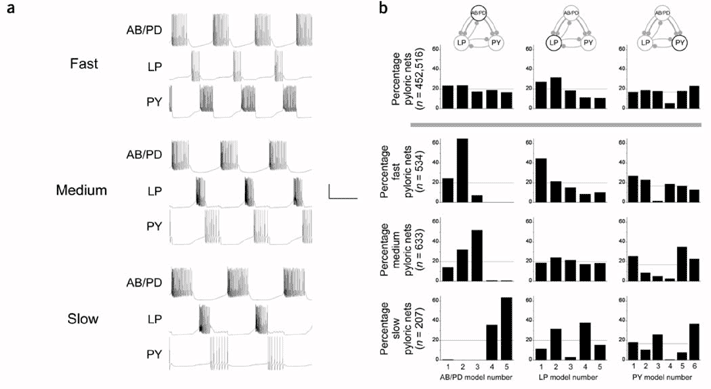
\includegraphics[width=1.0\linewidth]{gfx/Prinz6}
	\caption[Network degeneracy in model pyloric circuits.]{Network degeneracy in model pyloric circuits. (a) Voltage traces from simulated pyloric networks in fast, medium, and slow burst-frequency ranges. Scale bars, 1 s and 50 mV. (b) Percentages of pyloric networks that contain a given \acs{AB}-\acs{PD} model neuron (left), \acs{LP} model neuron (middle), or \acs{PY} model neuron (right). Top row, distributions for all pyloric networks; bottom rows, distributions for fast, medium and slow pyloric networks\autocite{PrinzSimilarnetworkactivity2004}.}
	\label{fig:prinz6}
\end{figure}

It has been demonstrated that there are many ways to produce stable, predictable output in models, as in animals, but these models have not been tested in response to modulation. Neuromodulation is a key way by which a neuronal circuit can be robust to unwelcome perturbation yet still respond with specialized activity when modulated. Network degeneracy comes secondary to this biological necessity.



